\documentclass{book}

\usepackage{float}
\usepackage{amsmath}
\usepackage{amsfonts}
\usepackage{graphicx}
\usepackage{lineno}
\usepackage{natbib}
\usepackage{hyperref}

\bibliographystyle{asa}

\floatstyle{plain}
\floatname{panel}{Panel}
\newfloat{algorithm}{h}{txt}[chapter]
\newfloat{panel}{h}{txt}[chapter]

\linenumbers

\begin{document}



\chapter{Introduction}
\label{chapt.intro}

\chapter{GLMS and WinBUGS}
\label{chapt.glms}

\chapter{Closed population models}
\label{chapt.closed}

\chapter{Fully Spatial capture-recapture models}
\label{chapt.scr0}

\chapter{Other observation models}
\label{chapt.poisson}

\chapter{MCMC details}
\label{chapt.mcmc}

\chapter{Goodness of Fit and stuff}
\label{chapt.gof}

\chapter{Covariate models}
\label{chapt.covariates}

\chapter{Inhomogeneous Point Process}
\label{chapt.ipp}

\chapter{Open models}
\label{chapt.open}


\chapter{Unmarked populations}
\label{chapt.unmarked}



\chapter{Spatial Capture-Recapture for Unmarked Populations}
\markboth{Chapter 14 }{}
\label{chapt.scr-unmarked}

\vspace{0.3cm}


Traditional capture-recapture models share the fundamental
assumption that each individual in a population can be uniquely
identified when captured. Often, this can be accomplished
by marking individuals with color bands, ear tags, or some other
artifical mark that can be subsequenly read in the field. For other
species, such as
tigers or marbled salamanders, individuals can be easily identified
using only their natural markings, yet many species
do not possess adequate natural markings and are
difficult to capture, making it impractical to use standard
capture-recapture techniques.

Estimating density when individuals are unmarked can be accomplished
using a variety of alternatives to capture-recapture, but many of
these methods have important limitations that warrant the exploration
of alternative approaches.
In this chapter we highlight the work of \citet{chandler_royle:2012}
who demonstrated that the ``individual recognition'' assumption of
capture-recapture models is not a requirement of spatial capture-recapture
models. They showed that, under certain conditions described below,
spatially-correlated count data are sufficient for
making inference about animal distribution and density even when no
individuals are marked.
The \citet{chandler_royle:2012} ``spatial count model'' (hereafter the
SC model) is virtually
identical to
other SCR models except that the encounter histories $\{z_{ijk}\}$ are not
directly
observed. Instead, the observed data are the counts realized by
summing up the detections for each individual at
a survey location during a sampling occasion $n_{jk} = \sum_i
z_{ijk}$.

The ability to fit
SCR models to data from unmarked populations has important
implications. For one, it means that SCR models can
be applied to data collected using methods like points counts in which
observers record simple counts of animals at an array of survey
points. Camera trapping data on unmarked animals such as deer or
coyotes could also also be suitable. In addition, this development has
important implications for
traditional SCR studies because many SCR datasets include some
individuals that cannnot be identified due to poor photo quality or
indistiguishable natural markings.

It is also interesting to note that by disregarding individual
identity, we wind up with a model that closely resembles another large
class of spatial models, known as convolution models
\citep{wolpert_ickstadt:1998,higdon:1998}. These
models have been used for a variety of purposes such as describing oceanic
surface temperatures and correlation in tree locations within managed
forests. The SC model offers an improvement in
some respects over existing convolution models because it does not
require arbitrary decisions about the location and number of ``support
points''. We will clarify this later in the chapter, and briefly
mention how this model can be used outside of SCR contexts for general
purpose spatial modeling of correlated count data.


\section{Existing Models for Inference About Density in Unmarked Populations}
\label{Sect.existing-unmarked}

When capture-recapture methods are not a viable option, researchers
often collect simple count data or even detection/non-detection data
to estimate population parameters. These data are often analyzed using
Poisson regression or logistic regression, perhaps with random
effects. When detection is imperfect, as it almost always is,
these methods cannot be used to obtain unbiased estimates of
population size or occurrence probability. Even when these data are
used an index of abundance or occurrence, standard models may yield
unreliable results when covariates affect both the state variable and
detection probability. A classic example is the finding by
\citet{bibby_buckland:1987} who reported that the detection
probability of
songbirds in restocked confier plantations was negatively associated
with vegetation height, yet population density was positively related to
vegetation height. This intuitive and common phenomenon has led to the
development of a vast number of models to estimate population size and
detection probability when individuals are unmarked. A review of these
models is beyond the scope of this
chapter, but we mention a few deficiencies of existing methods
that warrant the exploration of alternatives for robust inference when
standard capture-recapture methods do not apply.

Distance sampling \citep{buckland_etal:2001}, which we briefly
introduced in Chapter~\ref{chapt.intro},
is perhaps the most widely used method for
estimating population density when individuals are unmarked and
detection probability is less than one. This class of methods is known
to work impecibly when estimating the number of stakes in a field or
the number of duck nests in a wetland.
Distance sampling can also work very well in
more interesting situations, and is an extremely powerful method when
the assumptions can be met. However, the assumptions that distance
data can be recorded without error and that animals are distributed
randomly with respect to the transect can be easily violated by
common processes such as animal movement and measurement
error. Although numerous methods have been proposed to
relax some of these assumptions
\citet{royle_etal:2004, borchers_etal:1998, johnson_etal:2010,
  chandler_etal:2011},
another issue is that distance
sampling is simply not practical in many settings. For example, many
species are so rare and elusive that they can only be reliably
surveyed using methods such as camera traps.

Other common sampling methods used to estimate density when individuals are
unmarked include double-observer sampling, removal sampling, and
repeated counts, for which custom models have been developed
\citep{nichols_etal:2000, farnsworth_etal:2002, royle:2004,
  royle:2004abc,fiske_chandler:2011}. To
obtain reliable density estimates using these
methods, the area surveyed must be well defined and closed with
respect to movement and demographic processes. Given a short enough
sampling interval, such as a 5-min point-count, the closure
assumption may be reasonable. However, short sampling intervals limit
the number of detections, so observers generally visit each survey
location multiple times during a season. But then animal
movement may invalidate the closure assumption, and a model of
temporary emigration is required
\citep{kendall_etal:1997,chandler_etal:2011}. Furthermore,
distance-related heterogenity in detection probability can introduce
bias in these models, although this bias is negligible when the
ratio of plot size to the scale parameter of the detection function is low
\citep{efford_dawson:2009}.

We mention these issues not to suggest that
existing models do not have value---
indeed we believe that they can be used to obtain reliable density
estimates in many situations---rather our aim is to highlight the need for
alternative methods when the assumptions of existing methods cannot be
met. Additionally, the spatial count model we discuss in this chapter
serves as the
foundation for a broad class of SCR models in which all or some of the
individuals cannot be uniquely identified, which is the focus of the
next chapter.


\section{Spatial Correlation as Information}
\label{sect.corr-info}

All of the previous methods require some sort of auxiliary information
to seperately model abundance and detection. That is, we
need multiple observers or distance data or repeated visits to ensure
that model parameters are identifiable\footnote{Or we can make very
  strong model assumptions and get away without any auixiliary data
  \citep{lele_etal:2012, solymos_etal:2012}}. The same is true for
SC model \citep{chandler_royle:2012},
but the auxiliary information comes in the form of spatial
correlation, which requires no extra effort to collect.

It is natural to be suspicious of the claim that spatial correlation
is a good thing. Indeed, elaborate methods have been devised to deal
with spatial correlation as a nuisance parameter
\citep{dormann_etal:2007}, and ecologists have been admonisted for
failing to obtain ``real'' replicates uncontaminated by spatial
correlation \citep{hurlbert:1984}. The following heuristic may be
helpful.

Imagine a 10$\times$10 grid of camera traps and a single unmarked
individual
exposed to capture whose home range center lies in the center of the
trapping grid. If the individual has a small home range size relative
to the extent of the trapping grid, we can imagine what the
spatial correlation structure of the encounters might look
like. If the animal's movement is symmetric around the activity center
then the number of times the individual is detected at each
trap (the trap counts) is a function of the distance between the home
range center and the trap, \emph{i.e.} traps with the same distance
from the
activity center will yield counts that are more highly correlated with
one another than traps located at different distances from the
activity center. Thus, the correlation in counts tells us something
about the location of the activity center. It is relatively intuitive
that spatial correlation carries information about distribution, but
what about density?

Imagine now that there are two activity centers located in our traping
grid. Using trap counts alone, can our model tell us both where the
activity centers are and how many exist in the population exposed to
capture? The answer is yes, at least under certain circumstances.
Figure~\ref{ch14.fig.heur} illustrates the process. The map on the
left shows 500 simulated movement outcomes of the two individuals. The
right panel shows the total counts made at each trap after 10
survey occasions. Assuming that animals have bivariate normal home
ranges, the fact that there are two areas in the map with high counts
that dissipate in both dimensions suggests that the most likely number of
individuals given these data is 2. Furthermore, the degree to which
the counts dissipate from the two areas of highest intensity is
information about the home range size parameter $\sigma$. These two
piecies of information are enough to estimate density---again, given
that a bivariate normal home range is a valid assumption. Departures
from this assumption are discussed subsequently.

\begin{figure}
\centering
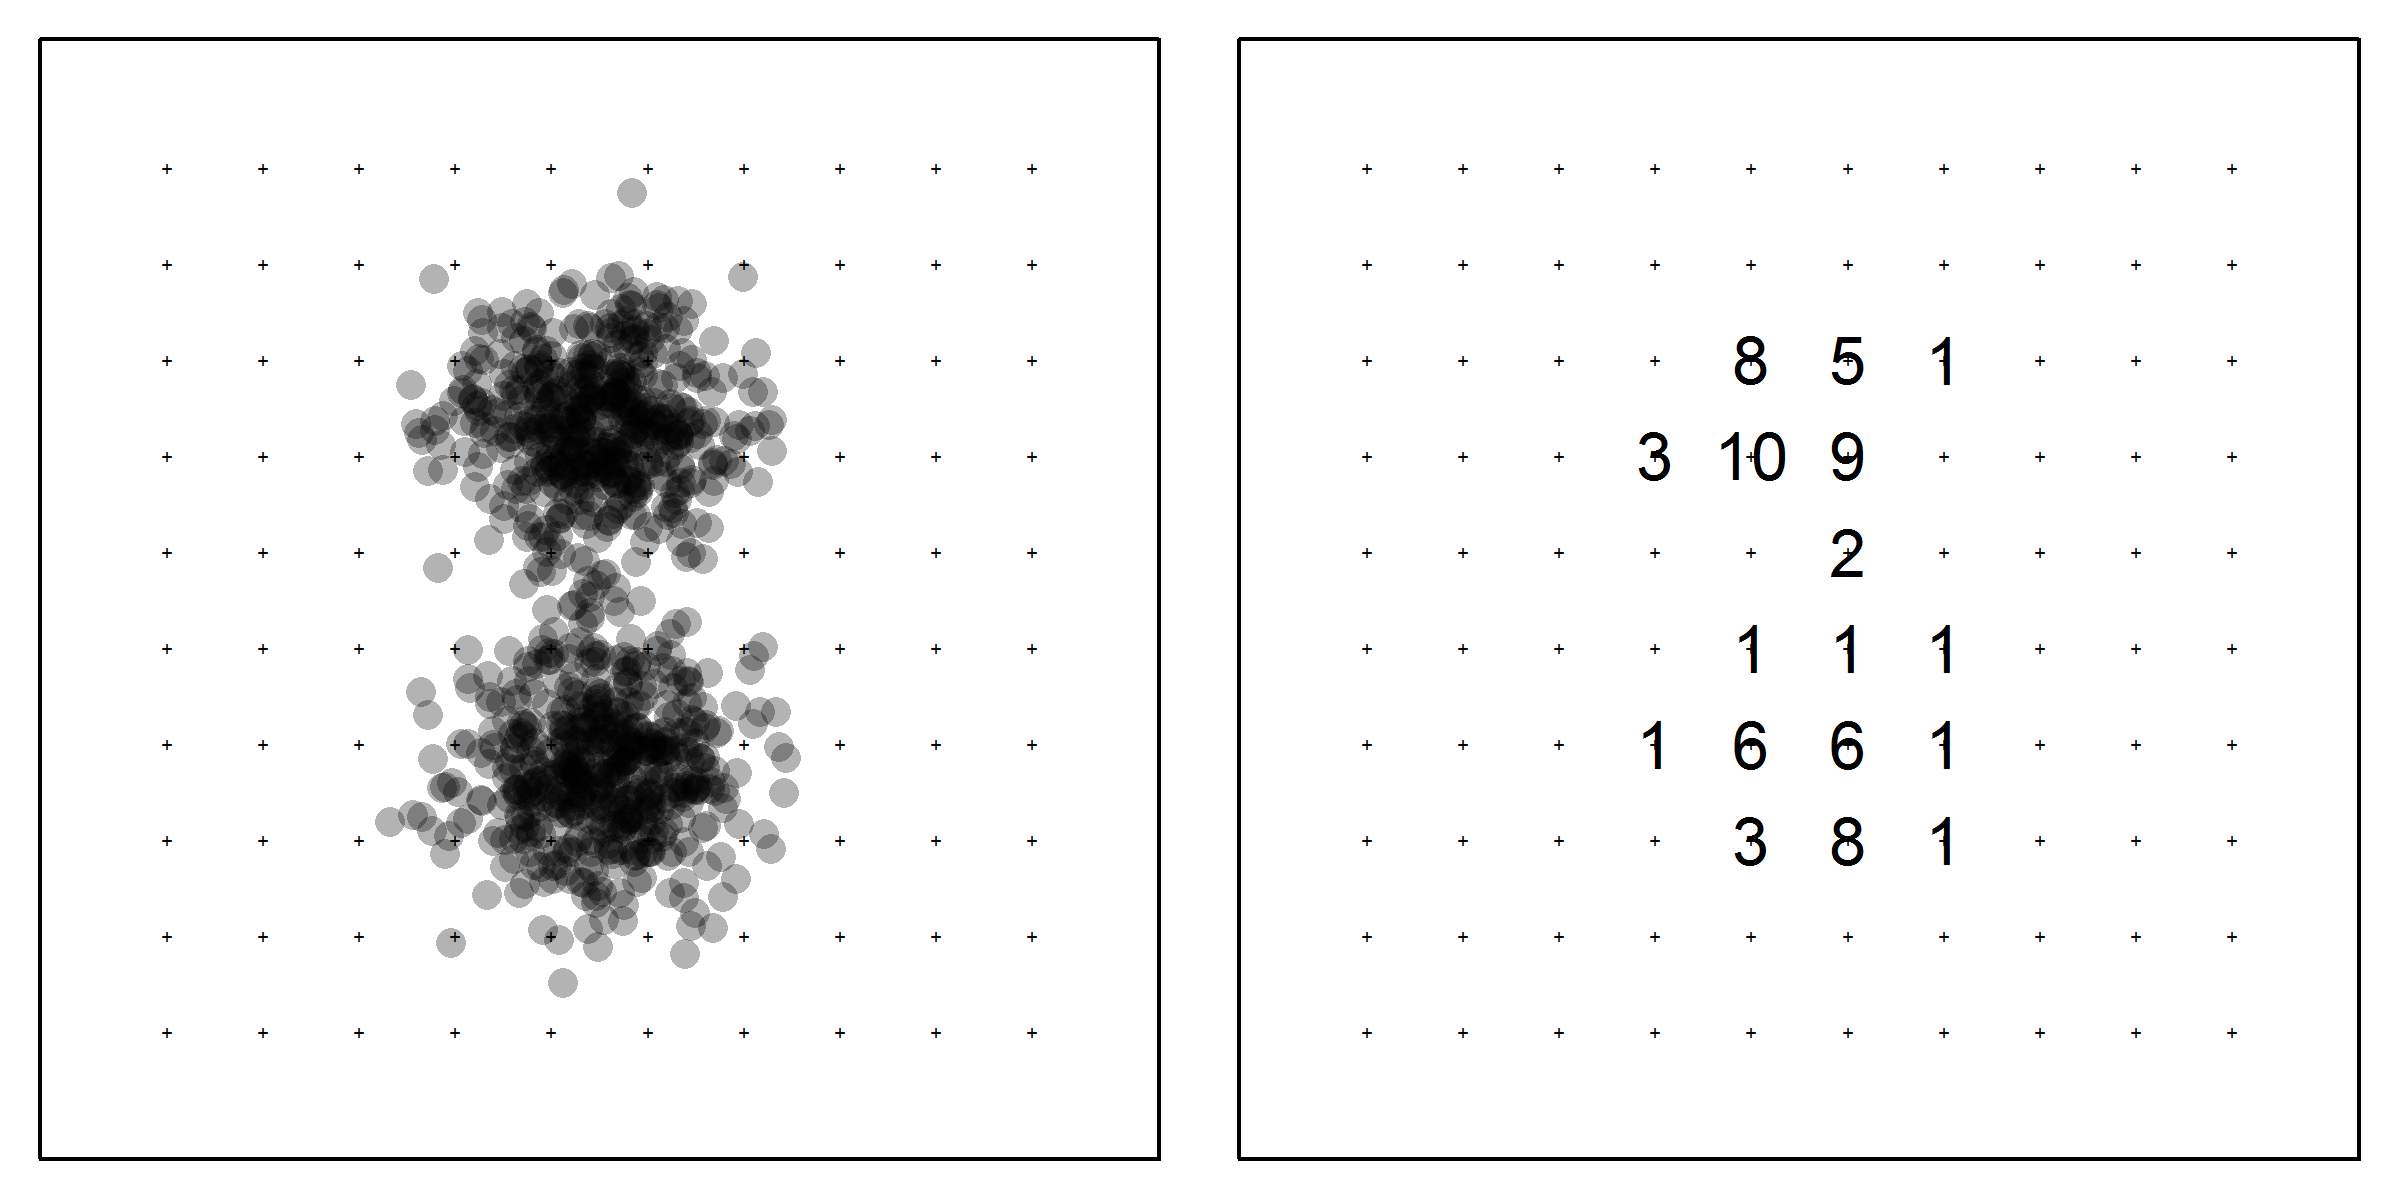
\includegraphics[width=4in,height=2in]{Ch14/figs/heuristic}
\caption{Movement outcomes (left) of two individuals with slightly
  overlapping home ranges. Crosses represent trap (or point count)
  locations. The right panel shows counts at each point. It is
  possible to estimate density using the count data alone.}
\label{ch14.fig.heur}
\end{figure}


\section{Data}

One of the important benefits of the SC model is that it
can be applied to data collected using an enormous variety of survey
methods. Whereas traditional SCR models require spatially-referenced
encounter histories, this model requires simple count data. Once
again, suppose that we have $J$ ``traps'' operated on $K$ time periods
during which no births or deaths occur. We use the term trap very
loosely in this context. A trap is simply some sampling device capable
of recording the number of individuals detected, $n_{jk}$, so traps could
be camera traps, hair snares, or even human observers standing at some
location $\bf x_j$. Regardless of the sampling method, the requisite
data are the counts $n_{jk}$ and the coordinates of the traps $\bf
x_j$. In some instances, we might have additional data such as
trap-specific covariates, state-space covariates, information on the
identities of a subset of individuals, or perhaps even distance
data. Some of these extensions are covered in
Chapters~\ref{chapt.partial} and~\ref{chapt.scrds}, but for the sake
of simplicity we focus on the basic data structure in this chapter.

\section{Model}


The state model that we
consider here is the same as in the basic spatial-capture setting,
in which we
we assume a homogeneous point process ${\bf s_i} \sim Unif(\cal{S})$
where $\bf s_i$ is the activity center of individual $i = 1,\dots,N$,
and $\cal{S}$ is the state-space which is typically a polygon defining
the region where the organism occur. This state model describes the
number and locations of animals. The observation model is once again
conditional on the state model and describes the encounter rate as a
function of the distance between activity centers and traps. At this
point in the book, we hope that you are thinking ``how could it be
otherwise? How could the probability of capture not be a function of
distance?'' If you are still skeptical and view this as an unrealistic
assmption rather than a truism, we encourage you to try to simulate
data in a more realistic fashion.

As with all SCR models, the encounter process is specific to the
sampling method, and here we consider the standard camera trapping
situation in which an
individual can be encountered at multiple traps during a single time
period, say one night during a camera-trapping study, and it can be
detected multiple times at a single trap during an occasion. This is
the Poisson encounter model described in
Chapter~\ref{chapt.obsmods}. The model for the capture histories can
be described by
\begin{equation}
 z_{ijk} \sim \mbox{Poisson}(\lambda_{ij}).
\label{eq.latentPoisson}
\end{equation}
where $\lambda_{ij}$ is the encounter rate
for individual $i$ at trap $j$. A common form of this parameter is
\[
\lambda_{ij} = \lambda_0 \exp(\| {\bf x_j - s_i} \| / 2\sigma^2)
\]
where $\lambda_0$ is the baseline encounter rate and $\sigma$ is the
scale parameter describing the distance-related decay in encounter
rate.

When individuals cannot be uniquely identified, the $z_{ijk}$ cannot
be directly observed, which seems like a massively insurmountable
problem. The solution is the same one we routinely apply when we
cannot directly observe the process of interest---we regard the
encounter histories as latent variables. The data are now just a
reduced-information
summary of the latent encounter histories. That is, they are the
sample- and trap-specific totals, aggregated over all individuals:
\[
n_{jk} = \sum_{i=1}^{N} z_{ijk}.
\]
This data structure, a matrix of counts made at a collection of
sampling locations on one or more occasions is extremely common in
ecology. Note also that we can get by with a single
occasion of data ($J \equiv 1$) because under the Poisson model,
\begin{equation}
n_{jk} \sim \mbox{Poisson}( \Lambda_{j} )
\label{eq:nagg}
\end{equation}
where
\[
 \Lambda_{j} = \lambda_0 \sum_{i} k_{ij},
\]
and because $\Lambda_r$ does not depend on $t$, we can
aggregate the replicated counts, defining
$n_{j.} = \sum_{k} n_{jk}$ and then
\[
 n_{j.} \sim \mbox{Poisson}( K \Lambda_{j} )
\]
As such, $K$ and $\lambda_{0}$ serve equivalent roles as affecting
baseline encounter rate as has been noted elsewhere
\citep{efford_etal:2009ecol}.


This formulation of the model in terms of the aggregate count
simplifies computations as the latent variables
$z_{irt}$ do not need to be updated in the MCMC estimation
scheme (see below). However, retaining $z_{irt}$
in the formulation of the model
is important if some individuals are uniquely marked, in which case
modifying
the MCMC algorithm to include both types of data is
trivial is straight-forward. This is because
uniquely identifiable individuals produce
observations of some of the $z_{irt}$ variables, which we elaborate
on in the subsequent chapter.






\section{Northern Parula Example}

Here we re-analyze the Northern Parula ({\it Parula americana}) data
described in \citet{chandler_royle:2012}. The data were collected at
105 points located on a 50-m grid at the Patuxent Wildlife Research
Center. Each point was surveyed 3 times during June 2006, and
Fig.~\ref{fig:nopaDat} depicts the resulting spatially-correlated
counts ($n_{r.}$).
A total of 226 detections were made with a maximum count of 4 during a
single survey. At 38 points, no warblers were detected. All but one of
the detections were of singing males, and this one observation was
not included in the analysis.


\begin{figure}
  \centering
  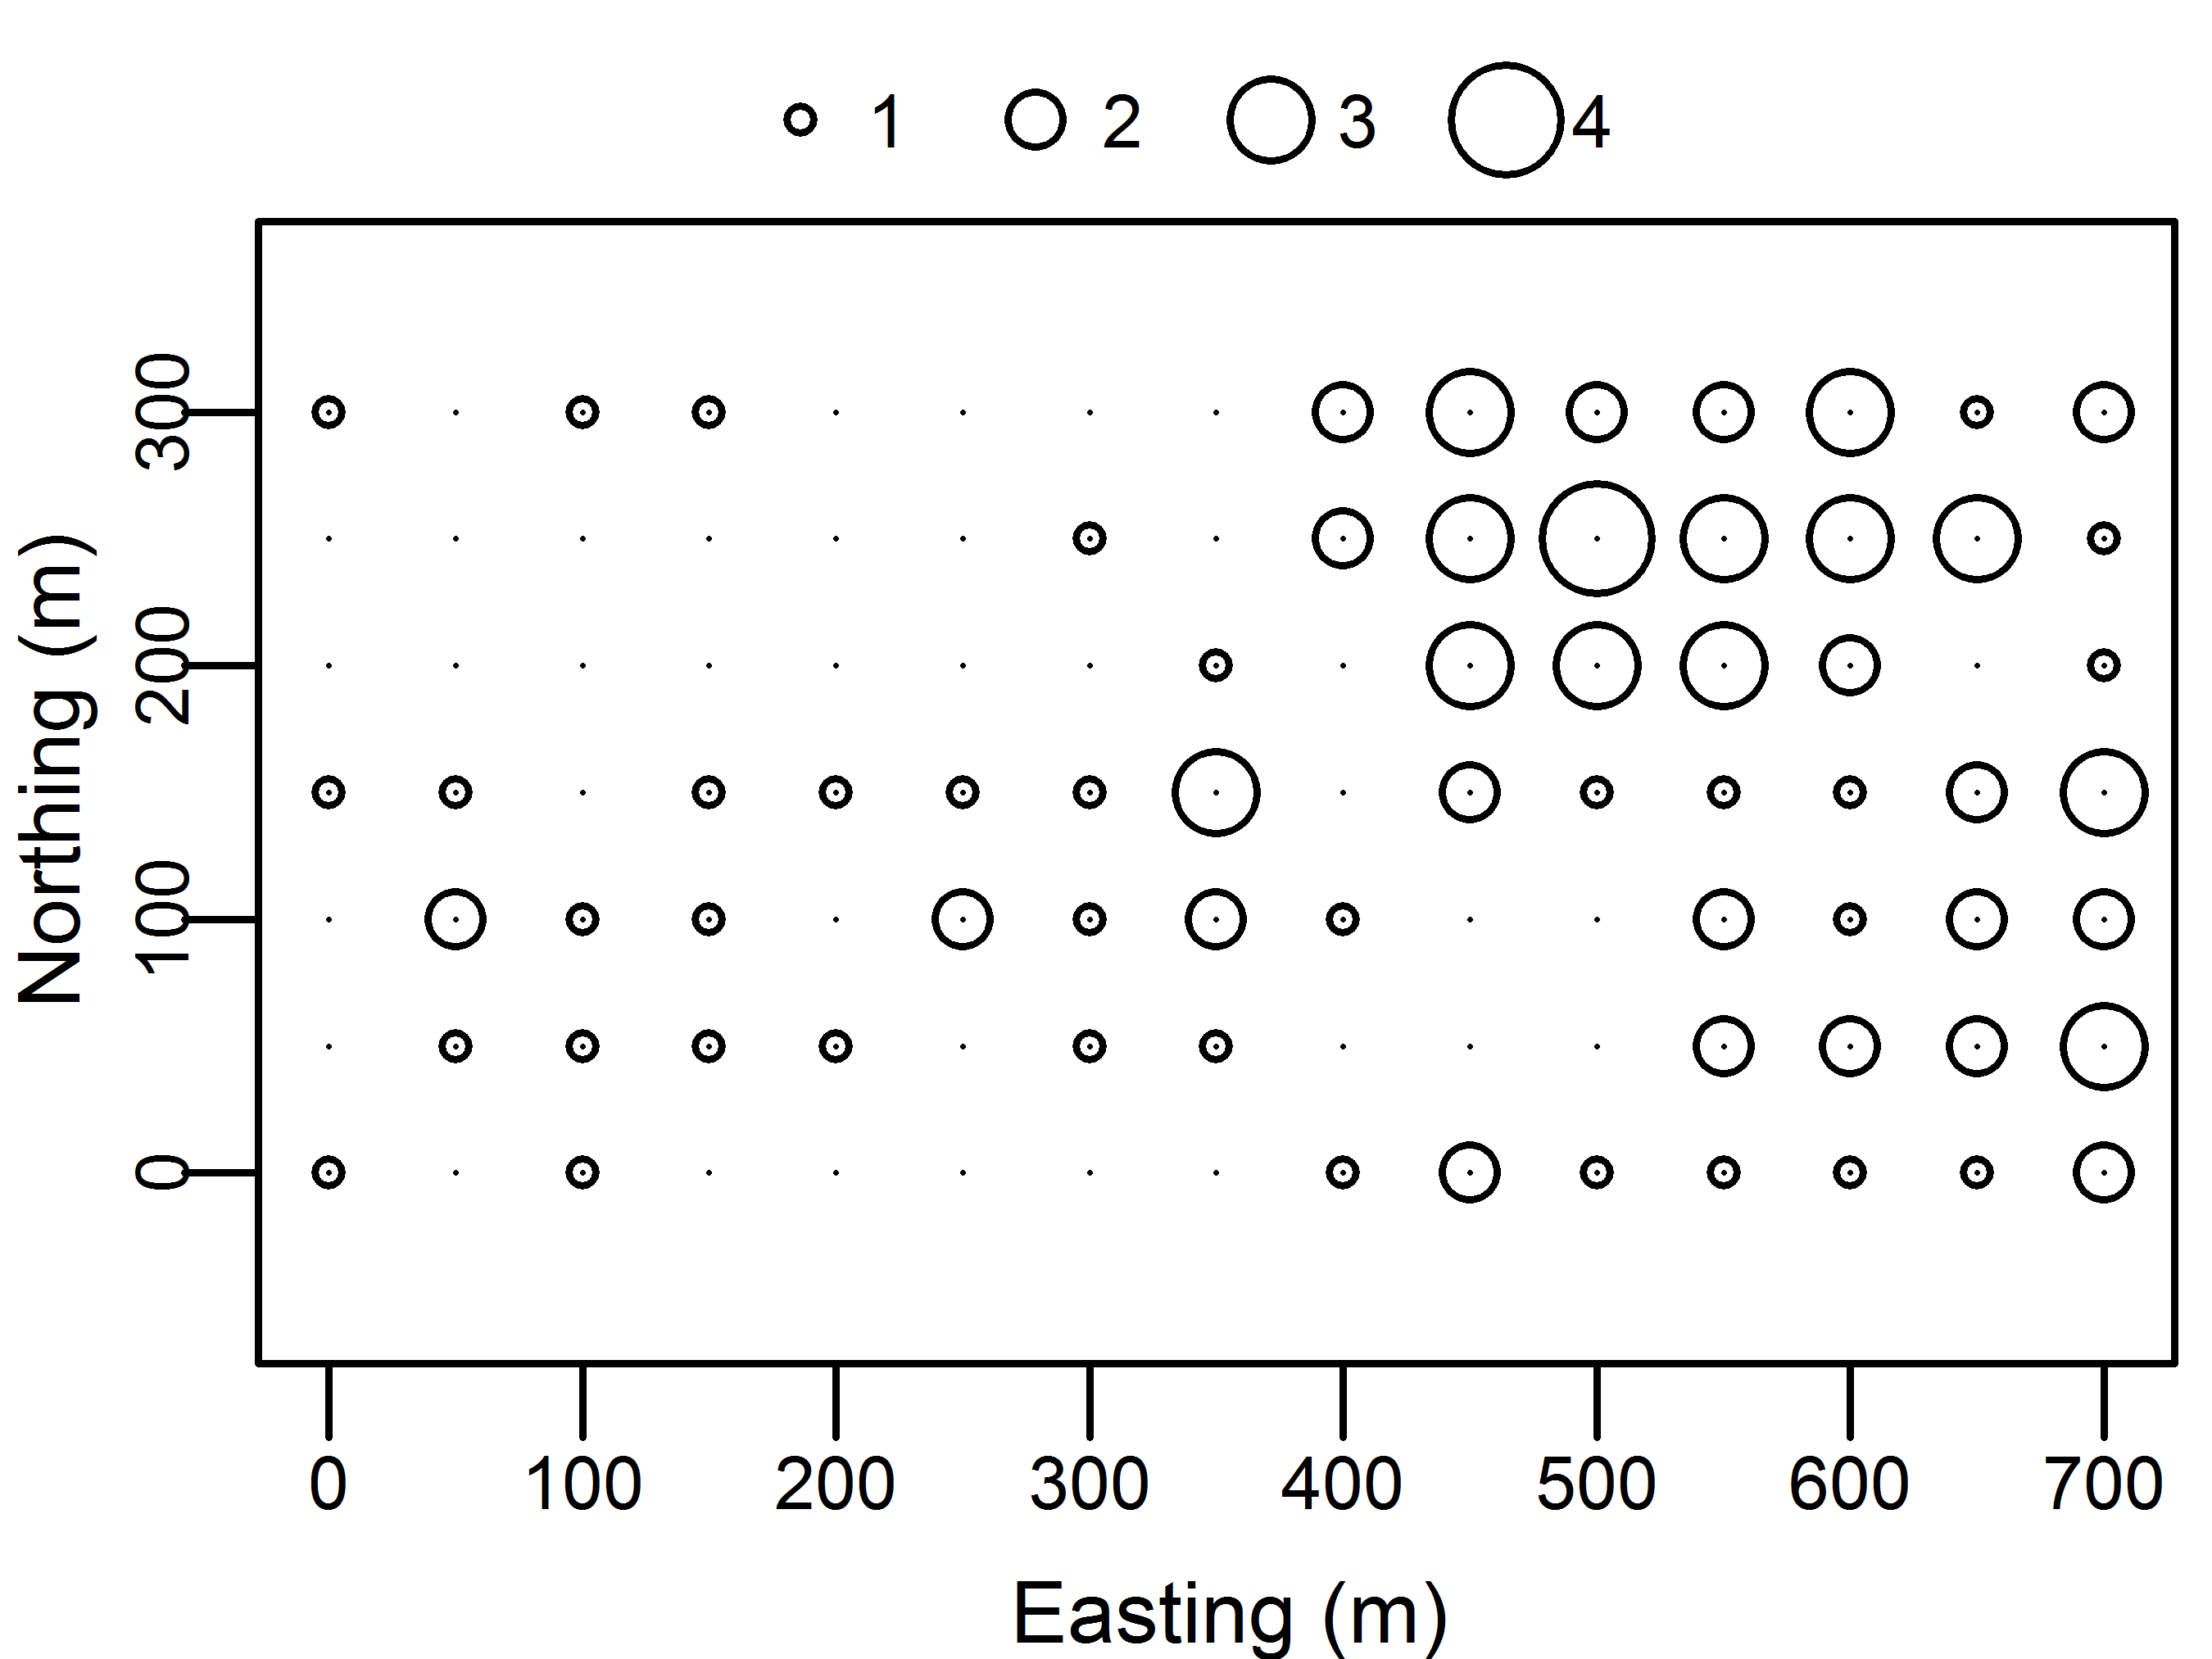
\includegraphics[width=3in,height=2.25in]{Ch14/figs/nopa}
  \caption{Spatially-correlated counts of northern parula on a 50-m
    grid. The size of the circle represents the total number of
    detections at each point.}
  \label{fig:nopaDat}
\end{figure}



In our analysis of the parula data, we defined the point process
state-space by buffering the grid of point
count locations by 250 m and used $M=300$.

At this point in time there is no canned software to fit this model,
and it is actually not straight-forward to use \bugs~because of the
constraints in the model\footnote{Although it can be done using the
  so-called ``ones-trick''}. However, \jags~has a neat distribution
called the \verb+dsum+ distribution, which was designed for this type
of situation where the observed data are a sum of random
variables. Remember, if we have 3 detections at a point, we assume
that these results as $\sum_i z_{ijk}$. Thus, we are summing up random
variables. \jags~actually works rather well for this situation
although it is quite slow. Another limitation of using \jags~is that
we can't mix data from marked and unmarked individuals because
\verb+dsum+ requires that we sum over unobserved quantities, not a mix
of observed and unobserved nodes. Thus, we can't use \jags~for the
situations considered in the next chapter, and thus we wrote our own
MCMC algorithm which overcomes these limitations, and it is somewhat
faster. Nonetheless, here is the \jags~code to analyze the NOPA data.

\begin{small}
\begin{verbatim}
model{
sigma ~ dunif(0, 5)
lam0 ~ dunif(0, 5)
psi ~ dunif(0, 1)
for(i in 1:M) {
   # Indicator of occurrence
   w[i] ~ dbern(psi)
   # Animal activity centers
   sx[i] ~ dunif(0, xSide)
   sy[i] ~ dunif(0, ySide)
   for(r in 1:nTraps) {
       # distance from plot center
       d[i, r] <- sqrt(pow(sx[i] - X[r, 1], 2) + pow(sy[i] - X[r, 2], 2))
       # encounter rate
       lam[i, r] <- lam0 * exp(-1*pow(d[i, r],2) / (2*pow(sigma,2))) * w[i]
       for(t in 1:nReps) {
           z[i, r, t] ~ dpois(lam[i, r])
           }
       }
   }
for(r in 1:nTraps) {
   for(t in 1:nReps) {
       y[r, t] ~ dsum(z[1,r,t],z[2,r,t], ... ,z[100,r,t]) # code abbreviated
       }
   }
N <- sum(w[])
}
\end{verbatim}
\end{small}

Note that this code will not run as shown because we abbreviated the
arguments to \verb+dsum+. In practice, you need to provide all 100 of
them, if $M=100$! This is kind of a drag, but you can easily create
the text using \verb+paste+ in \R. Maybe Martyn Plummer will throw us
a bone and allow for a vector as an argument. Anyhow, the entire
analysis is shown on the ???XX help page in \scrbook.


We simulated posterior
distributions using three Markov chains,
each consisting of 300000 iterations after discarding the initial 10000
draws. Convergence was satisfactory, as indicated by an $\hat{R}$
statistic of $<$ 1.02 \citep{gelman_rubin:1992}.


The posterior distribution for
$N$ was highly skewed with a long right tail resulting in a wide 95\%
credible interval (Table \ref{t:nopaPosts}). Nonetheless, the interval
for density, $D$, includes estimates reported from more intensive field
studies \citep{moldenhaer_regelski:1996}. As with any SCR model,
we can produce a density surface map, as shown in Fig.~\ref{fig:nopaDen}


\begin{table}%[t]
  \caption{Posterior summary statistics for spatial Poisson-count
    model applied to the northern parula data. Two sets of priors were
    considered. $M=300$ was used in both cases. Parulas/ha, $D$, is a
    derived parameter.}
  \scriptsize
  \begin{tabular}{l l rrrrrr}
    \hline
    Par        & Prior                  & Mean  & SD    & Mode   & q0.025  & q0.50  & q0.975  \\
    \hline
    $\sigma$   & $U(0, \infty)$   & 2.154   & 1.222  & 1.230   & 0.896   & 1.665   & 5.170    \\
    $\lambda_0$ & $U(0, \infty)$  & 0.284   & 0.149 & 0.212    & 0.084  & 0.256  & 0.665   \\
    $N$        & $U(0, M)$             & 40.953   & 38.072  & 4.000  & 3.000       & 31.000     & 143.000     \\
    $D$        &  --                   & 0.427    & 0.397 & 0.0417   & 0.0313  & 0.323  & 1.490    \\
    \hline
    $\sigma$    & $G(13, 10)$          & 1.301    & 0.258 & 1.230    & 0.889   & 1.266   & 1.908    \\
    $\lambda_0$ & $U(0, \infty)$ & 0.298    & 0.132 & 0.240    & 0.098   & 0.279  & 0.603   \\
    $N$         & $U(0, M)$            & 59.321   & 36.489  & 36.000 & 18.000      & 50.000     & 157.000     \\
    $D$         &  --                  & 0.618    & 0.380 & 0.375   & 0.188   & 0.521  & 1.635    \\
    \hline
  \end{tabular}
  \label{t:nopaPosts}
\vspace{0.5cm}
\end{table}


%\begin{comment}

\begin{figure}
  \centering
  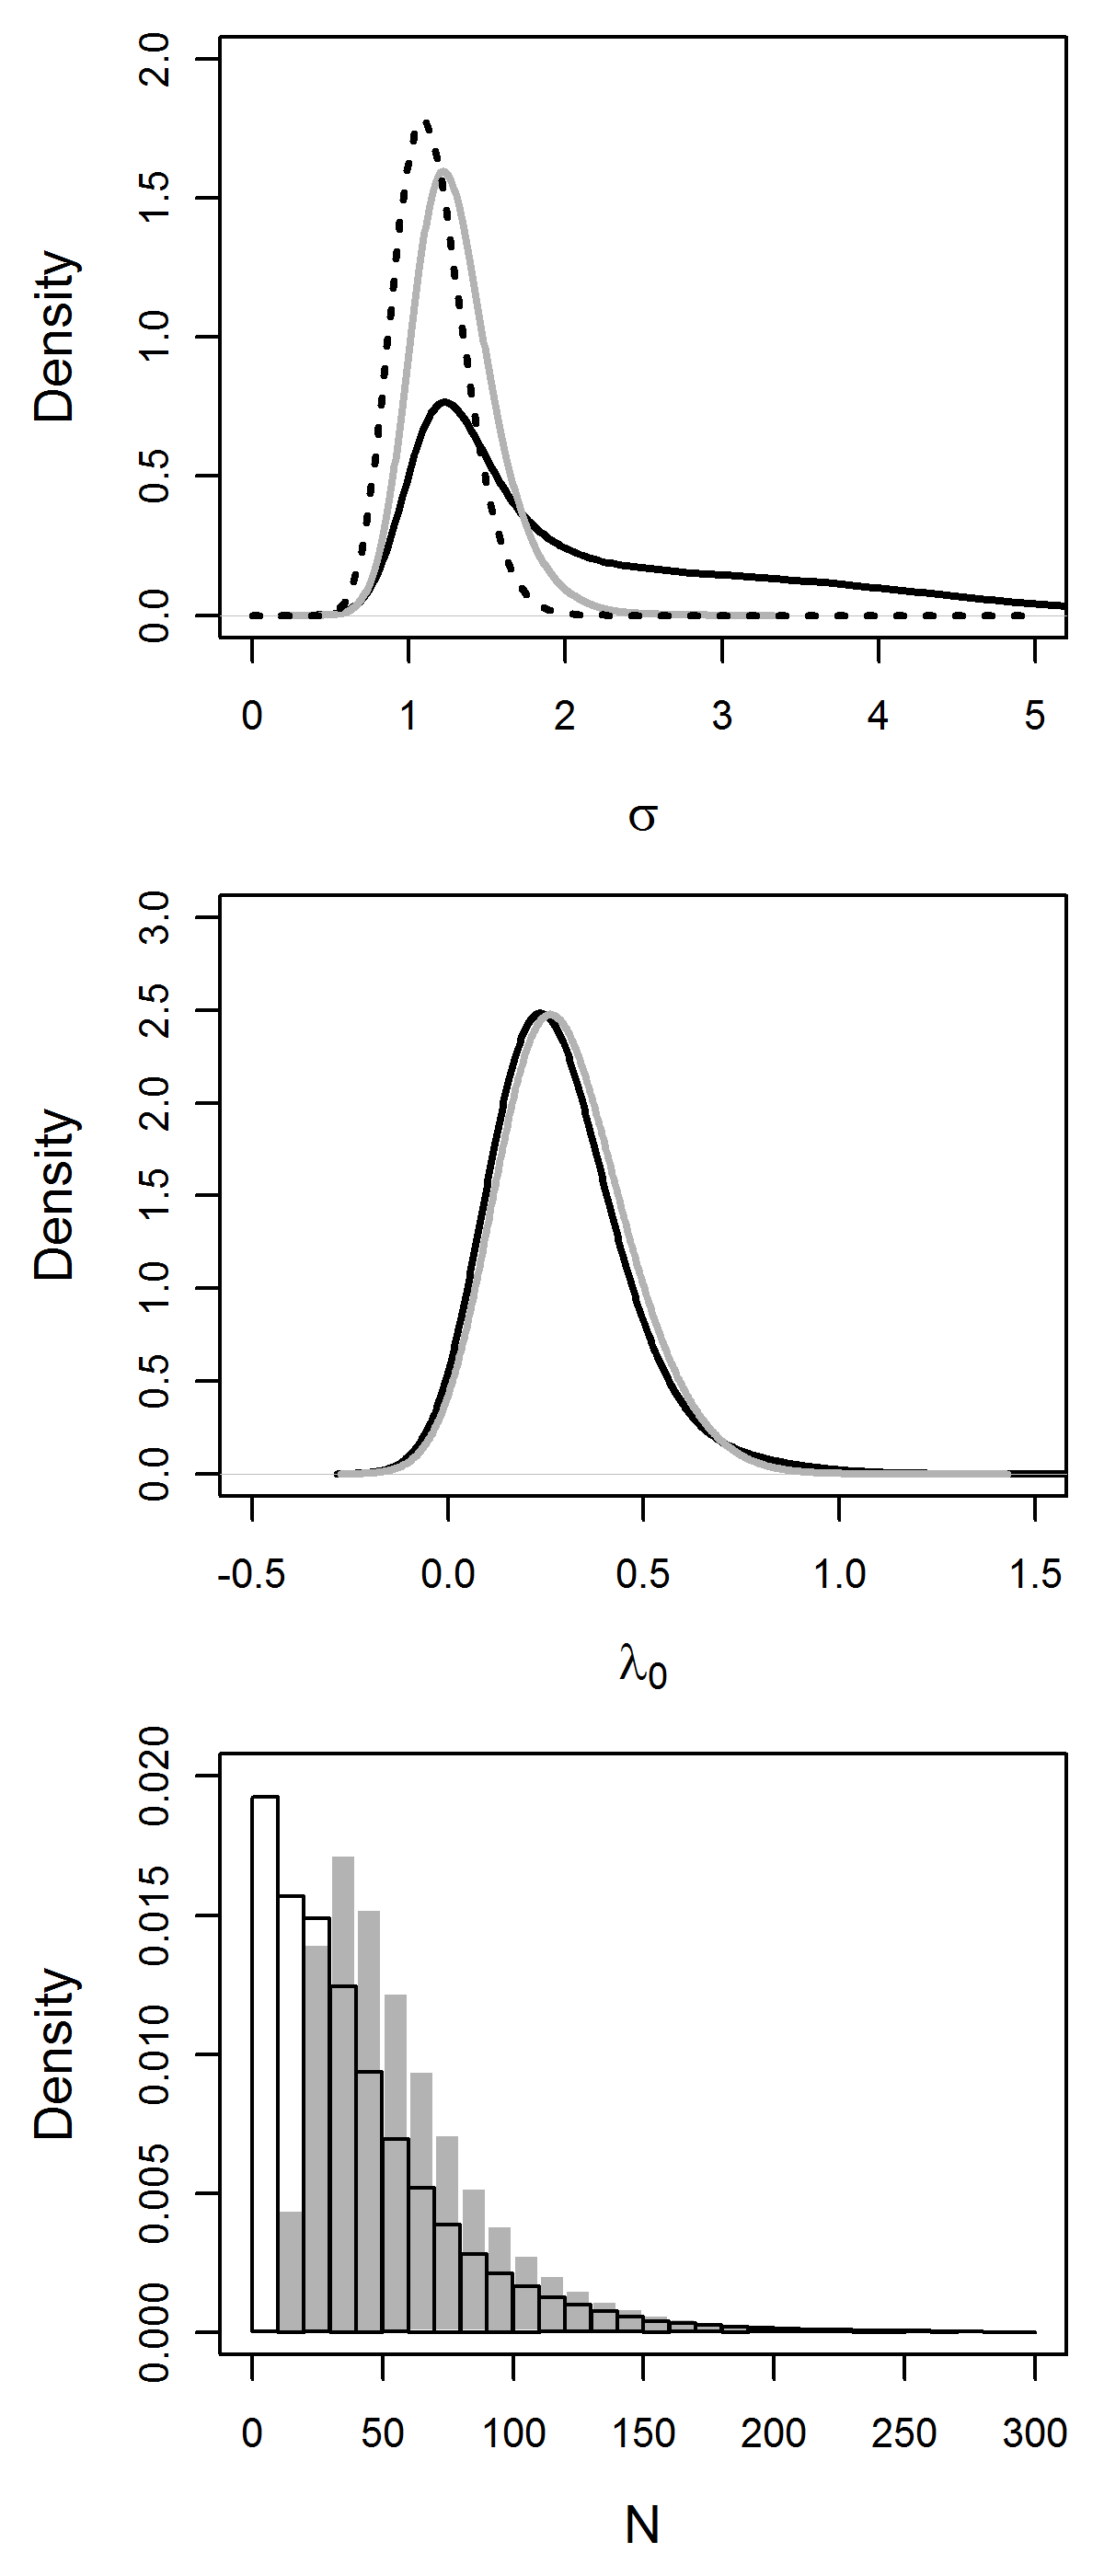
\includegraphics[width=1.5in,height=3in]{Ch14/figs/prior} % was 3,7
  \caption{Effects of $\sigma \sim \mbox{Gamma}(13,10)$
    prior on the posterior distributions from the northern parula
    model. Posteriors from model with uniform priors are
    shown in black, and posteriors from the informative prior model
    are shown in gray. The prior itself is shown as dotted line in the
    upper panel.}
  \label{fig:prior}
\end{figure}




\begin{figure}
  \centering
  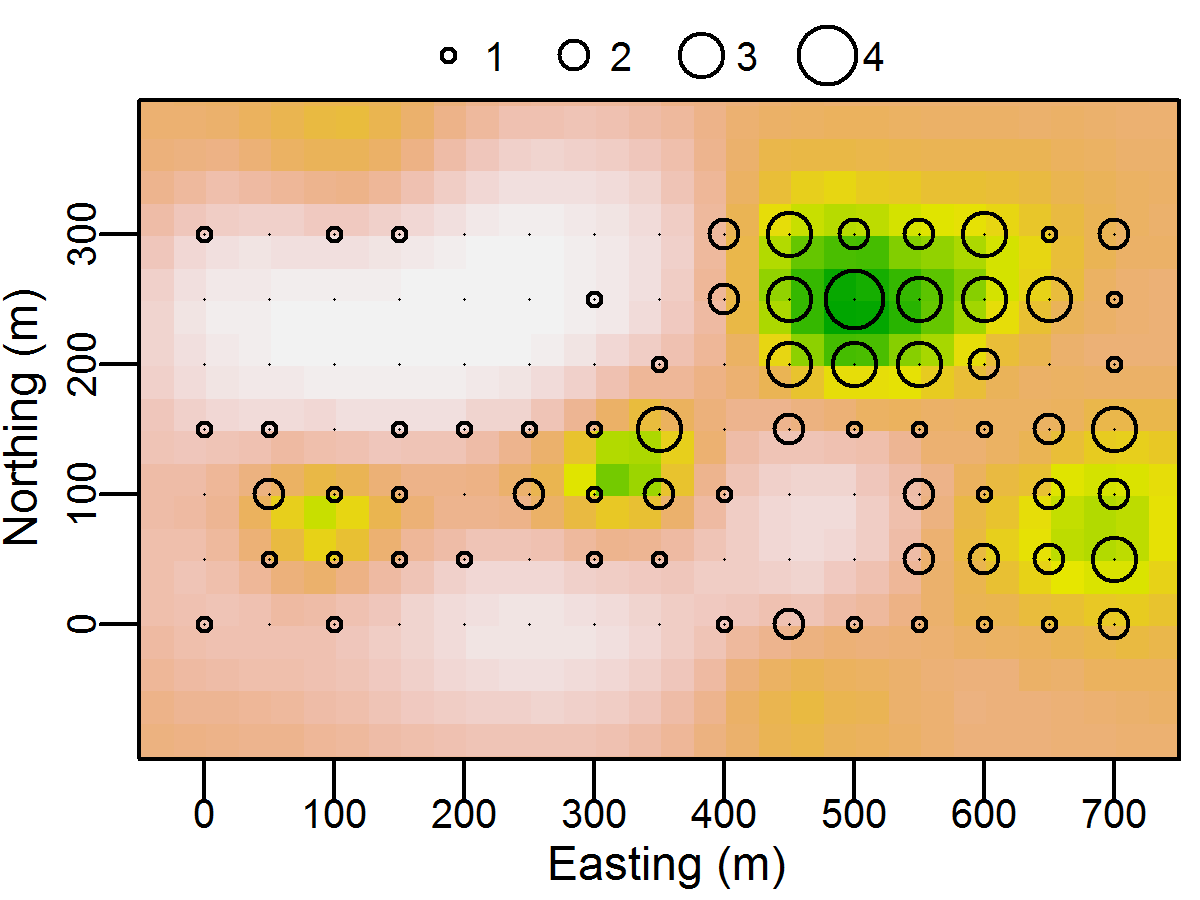
\includegraphics[width=3in,height=2.25in]{Ch14/figs/nopaDen}
  \caption{Estimated density surface of northern parula activity
    centers. The grid of point count locations with count totals is
    superimposed. See Fig. 1 for additional details.  }
  \label{fig:nopaDen}
\end{figure}

%\end{comment}



\section{Improving Precision with Prior Information}
\label{Sect.precision}

We are asking a lot of a little data. Because both the activity
centers and the encounter histories are latent variables, there is
inherently high uncertainty in the data, even if it is ``perfect''
data simulated from the true model. This explains the low posterior
precision in the parula data.

So why not just collect distance data or something? If you can, great---
we are not arguing against the use of other methods. But in many
cases, other models are not applicable. For instance, our model could
be applied to camera trapping data collected on species without
natural marks, such as pumas or coyotes. In addition, this
model provides an important foundation for modeling data where other
methods do not apply, and the underlying state model is so damn cool
because it corresponds to what we think is happening in the field.
Furthermore, the potential generalizations are numerous as we
will see later in this chapter and in the next chapter. In sum, the
model can be applied where no other models can, and it provides the
foundation for important extensions, but how can we improve precision?

Indeed, extensive information on home range size has
been compiled for many species in diverse habitats %\emph{e.g.}
\citep[\emph{e.g.},][]{degraaf_yamasaki:2001}. It is
easy to embody this information in a prior distribution as we
demonstrated for the parula data.


One benefit of a Bayesian analysis is that it can accommodate prior
information on the home range size and encounter rate parameters,
which are readily available for many
species. To illustrate, we analyzed the parula data using a new set of
priors. Whereas in the first analysis, all priors were
improper, customary non-informative priors (see Table \ref{t:nopaPosts}),
in the second set we used
an informative prior for the scale parameter $\sigma \sim
\mbox{Gamma}(13,10)$. We arrived at this prior using the methods
described by \citet{royle_etal:2011mee} and published
information on the warbler's home range size and detection probability
\citep{moldenhaer_regelski:1996,simons_etal:2009}. More details on this
derivation are found in ??????. We briefly note here that this prior
includes the biologically-plausible range of values from $\sigma$
suggested by the published literature.


This was true when
considering
both sets of priors, although posterior precision was higher under the
informative set of priors. Specifically, the use of prior information
reduced posterior density at high, biologically implausible,
values of $\sigma$, and hence decreased the posterior mass for
low values of $N$ (Fig.~\ref{fig:prior}).


\section{Design issues}

\subsection{How Much Correlation Is Enough?}

$\sigma$ shouldn't be too small or too large relative to trap spacing.

Can we test for correlation using K-functions or something?

\subsection{Linear Designs}

Survey points are not always located on a grid with even spacing---in
fact, it is rare to see a perfect 10$\times$10 grid of points in any
study because of habitat patchiness or rugged terrain or what have
you. Instead, points are often distributed haphazardly or using some form of
probability sampling. Such designs can still produce data amenable to
the models we consider in this chapter if individuals can be
encountered at multiple points, and none of the considerations
discussed above need to be modified. But what about linear designs?

In bird studies, point counts are often placed on linear transects. For
example, the Breeding Bird Survey involves surveying 50 points spaced
by 0.5 miles. The mountain-top bird survey in the White Mountain
National Forest involves surveying 42 transects, each with 20? points
spaced by 250-m \citep{king_etal:2008}. For many species, the 0.5 mile
spacing of the BBS will ensure that individuals are not detected at
multiple points. However, in the moutain-top survey, it's easy to
imagine that a Bicknell's Thrush (\emph{Catharus bicknelli}) could
easily be heard from adjacent points. So can we apply our model to
obtain density estimates with such simple counts?



\subsection{Quadrat counts}




\section{Other observation models}

Royle-Nichols model. What if we only have presence/absence data?

Will it work with a Binomial rather than a Poisson encounter model? I
don't think so










\subsection{Alternative Observation Models}
\label{Sect.alt-obsmods}

\citet{chandler_royle:2012} focused exclusively on the Poisson
observation model, but noted that alternative models such as the
Bernoulli model or the multinomial model (\ref{chapt.obsmods}) should
be easily accomodated.

When collecting DNA samples, for instance, an
individual can often be detected at most once during an
occasion, because multiple samples of biological material cannot be
attributed
to distinct episodes. Therefore, rather than $z_{irt} \sim Poisson(\lambda_{ir})$
we have $z_{irt} \sim Bernoulli(p_{ir})$ where, for example,  $p_{ir} = p_0
exp(-d_{ir}^2/(2\sigma^2))$, and $p_0$ is the probability of
detecting an individual whose home range is centered on trap $r$. This
Bernoulli model is a focus of ongoing investigations.

Both the Poisson and the Bernoulli models
produce count observations when aggregated over individuals to form
trap-specific totals; however, ecologists often collect so-called
``detection/non-detection'' data because it can be easier to determine
if ``at least one'' individual was present rather than enumerating all
individuals in a location. In this case, the underlying $z_{irt}$
array is the same as the above cases, but we observe $y_{rt} =
I(\sum_{i=1}^{N} z_{irt} > 0)$ where $I$ is the indicator
function. This ``Poisson-binary model'' is
a spatially explicit extension of the model of
\citet{royle_nichols:2003} in which the underlying abundance state
is inferred from binary data. We have investigated this model to a
limited extent but do not report on those results here.


\subsection{Spatial point process models}


Our model has some direct linkages to existing point process
models. We note that the observation intensity function (i.e.,
corresponding to the observation
locations) is a compound Gaussian kernel similar to
that of the Thomas process
\citep[pp. 61-62]{thomas:1949, moller_waagepetersen:2004}.
Also, the Poisson-Gamma Convolution models
\citep{wolpert_ickstadt:1998} are structurally similar (see also \cite{higdon:1998}
and \cite{best_etal:2000}).
 In particular, our model is such a model but
with a {\it constant} basal encounter rate $\lambda_{0}$
and {\it unknown} number and location of ``support points'', which in
our case are the animal activity centers, $\bf{s_i}$.
We can thus regard our model as a model for
{\it estimating} the location and local density of support points in
such models, which we believe could be useful in the application of
convolution models.  \citet{best_etal:2000} devise an MCMC algorithm for the
Poisson-Gamma model based on data augmentation, which is
similar to the component of our algorithm for
updating the $z$ variables in
the conditional-on-$z$ formulation of the model.  We emphasize that
our model is distinct from these Poisson-Gamma models
in that the number {\it and} location of such
support points are estimated.


If individuals were perfectly observable then the resulting point
process of locations is clearly a standard Poisson or Binomial (fixed
$N$) cluster process or Neyman-Scott process.
If detection is uniform over space but
imperfect, then the basic process is unaffected by this random thinning.
Our model can therefore be viewed formally as a Poisson (or Binomial)
cluster process model but one in which the thinning is
non-uniform, governed by the encounter model which dictates that
thinning rate increases with distance from the observation points. In
addition, our inference objective is, essentially, to estimate the
number of parents in the underlying Poisson cluster
process,
where the observations are biased by an incomplete sampling apparatus
(points in space).


As a model of a thinned point process, our model has much in common
with classical distance sampling models \citep{buckland_etal:2001}.
The main distinction is that our data structure does {\it not} include
observed distances, although the underlying observation model is
fundamentally the same as in distance sampling if there is only a
single replicate sample and $\bf{s}_i$ is defined as an individual's
location at an instant in time. For replicate samples, our model preserves
(latent) individuality across samples and traps which is not a feature
of distance sampling. We note that error in measurement of distance is
not a relevant consideration in our model, and we explicitly do not
require the standard distance sampling assumption that the probability
of detection is 1 if an individual occurs at the survey point. More
importantly, distance sampling models cannot be applied to data from
many of the sampling designs for which our model is relevant. For
example, many rare and endangered species can only be
effectively surveyed using methods such as hair snares and camera
traps that do not produce distance data \citep{oconnell_etal:2010}.


\section{Conclusion}

Concerns about ``statistical independence'' have prompted
ecologists to design count-based studies such that observed
random variables can be regarded as {\it i.i.d.} outcomes
\citep{hurlbert:1984}. Interestingly, this
often proves impossible in practice, and elaborate
methods have been devised to model spatial dependence as a nuisance
parameter. Our paper presents a modeling framework that directly
confronts this view by demonstrating that spatial
correlation carries information about the locations of individuals,
which can be used to estimate density even when individuals
are unmarked and distance-related heterogeneity exists in encounter
probability.






In this paper, we confronted one of the most difficult challenges
faced in wildlife sampling ---
estimation of density in the absence of data to distinguish among
individuals. To do so, we developed a novel class of
spatially-explicit models that
applies to spatially organized counts, where the count locations or
devices are located sufficiently close together so that individuals
are exposed to encounter at multiple devices. This design yields
correlation in the observed counts, and this correlation proves to be
informative about encounter probability parameters and hence density.
We note that sample locations in count-based studies are typically
{\it not} organized close
together in space because conventional wisdom and standard practice
dictate that independence of sample units is necessary
\citep{hurlbert:1984}. Our model
suggests that in some cases it might be advantageous to deviate from
the conventional wisdom if one is interested in direct inference about
density. Of course, this is also known in the application of standard spatial
capture-recapture  models \citep{borchers_efford:2008}
where individual
identity is preserved across trap encounters, but it is seldom, if
ever, considered in the design of more traditional count surveys.

Our model has broad relevance to an incredible number of animal
sampling problems. Our motivating problem involved bird point counts
where individual
identity is typically not available. The model also applies
to other standard methods used to sample unmarked
populations,  such as camera traps
or even methods that yield sign ({\it e.g.} scat, track) counts
indexed by space. However, results of our simulation study reveal some
important limitations of the basic
estimator applied to situations in which none of the individuals can
be uniquely identified. In particular, posterior
distributions are highly skewed in typical small to moderate sample
size situations and posterior precision is low.







\bibliography{AndyRefs_alphabetized}

\end{document}